% ======================================================================
%  Somantha Manuranga - Master CV (English)
%
%  This is the MASTER version: it lists everything. For a specific
%  application, copy this file and delete the projects and lines that do
%  not match the job advert, aiming for two pages.
%
%  Build:  pdflatex cv-en.tex   (run twice for the page count)
%     or:  npm run cv           (from the repository root; builds EN + DE)
%  Layout and personal data: cv-style.tex
% ======================================================================
\documentclass[a4paper,10pt]{article}

\newcommand{\cvlang}{english}
\newcommand{\cvpdflang}{en-GB}
\newcommand{\cvdoctitle}{Curriculum Vitae}
\newcommand{\cvpageword}{Page}
% ======================================================================
%  Shared style for the master CV (cv-en.tex and cv-de.tex)
%
%  Layout follows the previous CV (Jake Gutierrez's resume template, MIT
%  licence), adapted to A4 and tuned for applicant tracking systems (ATS):
%    - one column, standard section names, real text only
%    - no icon fonts (they extract as garbage characters)
%    - every glyph mapped to Unicode, f-ligatures switched off
%    - PDF title, author and keywords set
%
%  Before % ======================================================================
%  Shared style for the master CV (cv-en.tex and cv-de.tex)
%
%  Layout follows the previous CV (Jake Gutierrez's resume template, MIT
%  licence), adapted to A4 and tuned for applicant tracking systems (ATS):
%    - one column, standard section names, real text only
%    - no icon fonts (they extract as garbage characters)
%    - every glyph mapped to Unicode, f-ligatures switched off
%    - PDF title, author and keywords set
%
%  Before % ======================================================================
%  Shared style for the master CV (cv-en.tex and cv-de.tex)
%
%  Layout follows the previous CV (Jake Gutierrez's resume template, MIT
%  licence), adapted to A4 and tuned for applicant tracking systems (ATS):
%    - one column, standard section names, real text only
%    - no icon fonts (they extract as garbage characters)
%    - every glyph mapped to Unicode, f-ligatures switched off
%    - PDF title, author and keywords set
%
%  Before \input{cv-style} the main file must define:
%    \cvlang      babel language (english or ngerman)
%    \cvpdflang   PDF language tag (en-GB or de-DE)
%    \cvdoctitle  document title for the PDF metadata
%    \cvpageword  the word for "page" in the footer
% ======================================================================

\usepackage[T1]{fontenc}
\usepackage[utf8]{inputenc}
\usepackage[\cvlang]{babel}
\usepackage{lmodern}
\usepackage[a4paper,left=1.45cm,right=1.45cm,top=1.1cm,bottom=1.45cm,footskip=0.7cm]{geometry}
\usepackage{titlesec}
\usepackage{enumitem}
\usepackage{graphicx}
\usepackage{xcolor}
\usepackage{fancyhdr}
\usepackage{lastpage}
\usepackage{microtype}
\usepackage[hidelinks]{hyperref}

% ---------- ATS: machine-readable text ----------
\input{glyphtounicode}
\pdfgentounicode=1
\DisableLigatures[f]{encoding = *, family = *}

% ---------- Personal data (edit once, used by both languages) ----------
\newcommand{\cvname}{Somantha Manuranga}
\newcommand{\cvphone}{+49 174 7656939}
\newcommand{\cvemail}{somanthamanuranga@gmail.com}
\newcommand{\cvlinkedin}{linkedin.com/in/somantha-manuranga-b73432192}
\newcommand{\cvgithub}{github.com/SomanthaManuranga}
\newcommand{\cvportfolio}{somanthamanuranga.github.io/portfolio}

% Set to \photofalse for a version without a photo (some online
% application forms and international employers prefer that).
\newif\ifphoto
\phototrue

\hypersetup{
  pdftitle={\cvname\ - \cvdoctitle},
  pdfauthor={\cvname},
  pdfsubject={\cvdoctitle},
  pdfkeywords={AI Engineer, Machine Learning, Deep Learning, Computer Vision, NLP, LLM, PyTorch, Python, Industrial AI, Werkstudent},
  pdflang={\cvpdflang},
}

% ---------- Page ----------
\pagestyle{fancy}
\fancyhf{}
\renewcommand{\headrulewidth}{0pt}
\renewcommand{\footrulewidth}{0pt}
\fancyfoot[C]{\footnotesize\color{black!55}\cvname\ \textperiodcentered\ \cvpageword\ \thepage\ / \pageref*{LastPage}}
\setlength{\parindent}{0pt}
\setlength{\tabcolsep}{0pt}
\raggedbottom
\raggedright
\urlstyle{same}

% ---------- Section headings: small caps with a rule ----------
\titleformat{\section}{\vspace{-5pt}\scshape\raggedright\large}{}{0em}{}[\color{black}\titlerule\vspace{-5pt}]
\titlespacing*{\section}{0pt}{9pt}{7pt}

% ---------- Building blocks ----------
% \cvheader{line 1}{line 2}{line 3}{line 4}
% Each contact detail sits in an \mbox so that it is never hyphenated or
% split across lines (a broken email address or URL confuses ATS parsers).
\newcommand{\cvheader}[4]{%
  \begin{minipage}[c]{0.78\textwidth}
    {\Huge\bfseries \cvname}\\[6pt]
    {\small #1}\\[1.5pt]
    {\small #2}\\[1.5pt]
    {\small #3}\\[1.5pt]
    {\small #4}
  \end{minipage}%
  \hfill
  \ifphoto
  \begin{minipage}[c]{0.19\textwidth}
    \raggedleft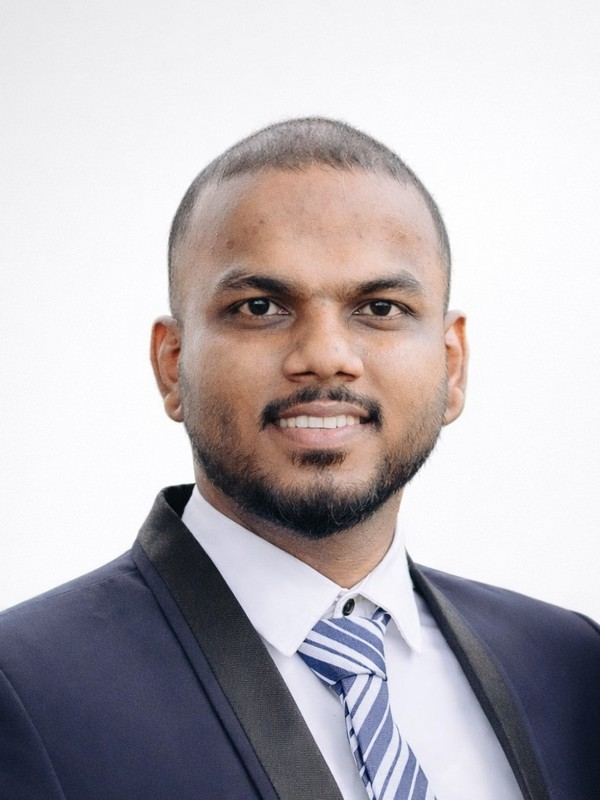
\includegraphics[width=2.75cm]{photo.jpg}
  \end{minipage}%
  \fi
  \par\vspace{3pt}
}
\newcommand{\cvsep}{\hspace{5pt}\textbullet\hspace{5pt}}

% Entry lists
\newcommand{\cvliststart}{\begin{itemize}[leftmargin=0.25cm, label={}, itemsep=3pt, topsep=0pt, parsep=0pt]}
\newcommand{\cvlistend}{\end{itemize}}

% \cventry{organisation}{location}{role or degree}{dates}
\newcommand{\cventry}[4]{%
  \item
  \begin{tabular*}{\linewidth}[t]{l@{\extracolsep{\fill}}r}
    \textbf{#1} & {\small #2} \\
    \textit{\small #3} & \textit{\small #4} \\
  \end{tabular*}\nopagebreak\vspace{-2pt}
}

% \cvproject{name}{technologies}{year}
\newcommand{\cvproject}[3]{%
  \item
  \begin{tabular*}{\linewidth}[t]{l@{\extracolsep{\fill}}r}
    {\small\textbf{#1} $|$ \textit{#2}} & \textit{\small #3} \\
  \end{tabular*}\nopagebreak\vspace{-2pt}
}

% \cvgroup{label}: sub-heading inside the project list
\newcommand{\cvgroup}[1]{\item[] \vspace{1pt}{\small\bfseries\itshape #1}\vspace{-1pt}}

% Bullet points under an entry
\newcommand{\cvpointsstart}{\begin{itemize}[leftmargin=0.45cm, label=\textbullet, itemsep=0.5pt, topsep=1pt, parsep=0pt]\small}
\newcommand{\cvpointsend}{\end{itemize}}

% \cvline{label}{text}: one line in the skills-style sections
\newcommand{\cvline}[2]{\item {\small \textbf{#1:} #2}}
 the main file must define:
%    \cvlang      babel language (english or ngerman)
%    \cvpdflang   PDF language tag (en-GB or de-DE)
%    \cvdoctitle  document title for the PDF metadata
%    \cvpageword  the word for "page" in the footer
% ======================================================================

\usepackage[T1]{fontenc}
\usepackage[utf8]{inputenc}
\usepackage[\cvlang]{babel}
\usepackage{lmodern}
\usepackage[a4paper,left=1.45cm,right=1.45cm,top=1.1cm,bottom=1.45cm,footskip=0.7cm]{geometry}
\usepackage{titlesec}
\usepackage{enumitem}
\usepackage{graphicx}
\usepackage{xcolor}
\usepackage{fancyhdr}
\usepackage{lastpage}
\usepackage{microtype}
\usepackage[hidelinks]{hyperref}

% ---------- ATS: machine-readable text ----------
\input{glyphtounicode}
\pdfgentounicode=1
\DisableLigatures[f]{encoding = *, family = *}

% ---------- Personal data (edit once, used by both languages) ----------
\newcommand{\cvname}{Somantha Manuranga}
\newcommand{\cvphone}{+49 174 7656939}
\newcommand{\cvemail}{somanthamanuranga@gmail.com}
\newcommand{\cvlinkedin}{linkedin.com/in/somantha-manuranga-b73432192}
\newcommand{\cvgithub}{github.com/SomanthaManuranga}
\newcommand{\cvportfolio}{somanthamanuranga.github.io/portfolio}

% Set to \photofalse for a version without a photo (some online
% application forms and international employers prefer that).
\newif\ifphoto
\phototrue

\hypersetup{
  pdftitle={\cvname\ - \cvdoctitle},
  pdfauthor={\cvname},
  pdfsubject={\cvdoctitle},
  pdfkeywords={AI Engineer, Machine Learning, Deep Learning, Computer Vision, NLP, LLM, PyTorch, Python, Industrial AI, Werkstudent},
  pdflang={\cvpdflang},
}

% ---------- Page ----------
\pagestyle{fancy}
\fancyhf{}
\renewcommand{\headrulewidth}{0pt}
\renewcommand{\footrulewidth}{0pt}
\fancyfoot[C]{\footnotesize\color{black!55}\cvname\ \textperiodcentered\ \cvpageword\ \thepage\ / \pageref*{LastPage}}
\setlength{\parindent}{0pt}
\setlength{\tabcolsep}{0pt}
\raggedbottom
\raggedright
\urlstyle{same}

% ---------- Section headings: small caps with a rule ----------
\titleformat{\section}{\vspace{-5pt}\scshape\raggedright\large}{}{0em}{}[\color{black}\titlerule\vspace{-5pt}]
\titlespacing*{\section}{0pt}{9pt}{7pt}

% ---------- Building blocks ----------
% \cvheader{line 1}{line 2}{line 3}{line 4}
% Each contact detail sits in an \mbox so that it is never hyphenated or
% split across lines (a broken email address or URL confuses ATS parsers).
\newcommand{\cvheader}[4]{%
  \begin{minipage}[c]{0.78\textwidth}
    {\Huge\bfseries \cvname}\\[6pt]
    {\small #1}\\[1.5pt]
    {\small #2}\\[1.5pt]
    {\small #3}\\[1.5pt]
    {\small #4}
  \end{minipage}%
  \hfill
  \ifphoto
  \begin{minipage}[c]{0.19\textwidth}
    \raggedleft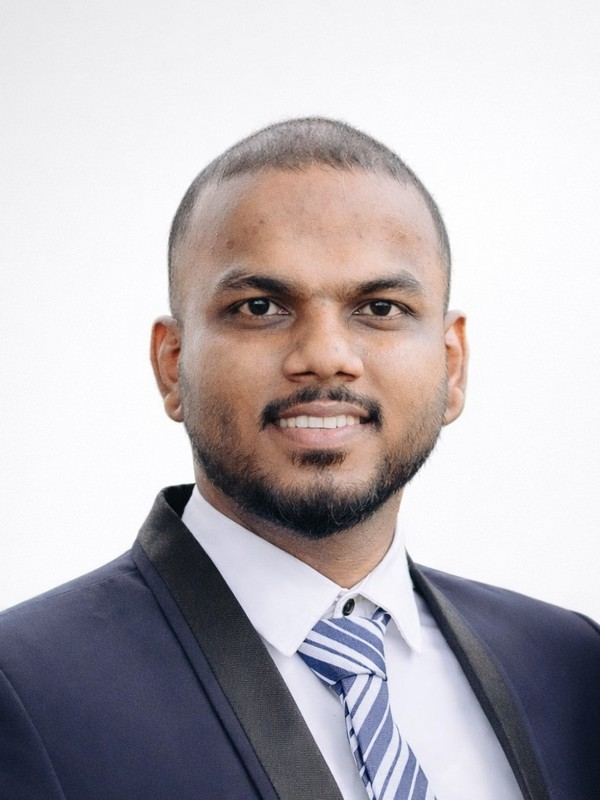
\includegraphics[width=2.75cm]{photo.jpg}
  \end{minipage}%
  \fi
  \par\vspace{3pt}
}
\newcommand{\cvsep}{\hspace{5pt}\textbullet\hspace{5pt}}

% Entry lists
\newcommand{\cvliststart}{\begin{itemize}[leftmargin=0.25cm, label={}, itemsep=3pt, topsep=0pt, parsep=0pt]}
\newcommand{\cvlistend}{\end{itemize}}

% \cventry{organisation}{location}{role or degree}{dates}
\newcommand{\cventry}[4]{%
  \item
  \begin{tabular*}{\linewidth}[t]{l@{\extracolsep{\fill}}r}
    \textbf{#1} & {\small #2} \\
    \textit{\small #3} & \textit{\small #4} \\
  \end{tabular*}\nopagebreak\vspace{-2pt}
}

% \cvproject{name}{technologies}{year}
\newcommand{\cvproject}[3]{%
  \item
  \begin{tabular*}{\linewidth}[t]{l@{\extracolsep{\fill}}r}
    {\small\textbf{#1} $|$ \textit{#2}} & \textit{\small #3} \\
  \end{tabular*}\nopagebreak\vspace{-2pt}
}

% \cvgroup{label}: sub-heading inside the project list
\newcommand{\cvgroup}[1]{\item[] \vspace{1pt}{\small\bfseries\itshape #1}\vspace{-1pt}}

% Bullet points under an entry
\newcommand{\cvpointsstart}{\begin{itemize}[leftmargin=0.45cm, label=\textbullet, itemsep=0.5pt, topsep=1pt, parsep=0pt]\small}
\newcommand{\cvpointsend}{\end{itemize}}

% \cvline{label}{text}: one line in the skills-style sections
\newcommand{\cvline}[2]{\item {\small \textbf{#1:} #2}}
 the main file must define:
%    \cvlang      babel language (english or ngerman)
%    \cvpdflang   PDF language tag (en-GB or de-DE)
%    \cvdoctitle  document title for the PDF metadata
%    \cvpageword  the word for "page" in the footer
% ======================================================================

\usepackage[T1]{fontenc}
\usepackage[utf8]{inputenc}
\usepackage[\cvlang]{babel}
\usepackage{lmodern}
\usepackage[a4paper,left=1.45cm,right=1.45cm,top=1.1cm,bottom=1.45cm,footskip=0.7cm]{geometry}
\usepackage{titlesec}
\usepackage{enumitem}
\usepackage{graphicx}
\usepackage{xcolor}
\usepackage{fancyhdr}
\usepackage{lastpage}
\usepackage{microtype}
\usepackage[hidelinks]{hyperref}

% ---------- ATS: machine-readable text ----------
\input{glyphtounicode}
\pdfgentounicode=1
\DisableLigatures[f]{encoding = *, family = *}

% ---------- Personal data (edit once, used by both languages) ----------
\newcommand{\cvname}{Somantha Manuranga}
\newcommand{\cvphone}{+49 174 7656939}
\newcommand{\cvemail}{somanthamanuranga@gmail.com}
\newcommand{\cvlinkedin}{linkedin.com/in/somantha-manuranga-b73432192}
\newcommand{\cvgithub}{github.com/SomanthaManuranga}
\newcommand{\cvportfolio}{somanthamanuranga.github.io/portfolio}

% Set to \photofalse for a version without a photo (some online
% application forms and international employers prefer that).
\newif\ifphoto
\phototrue

\hypersetup{
  pdftitle={\cvname\ - \cvdoctitle},
  pdfauthor={\cvname},
  pdfsubject={\cvdoctitle},
  pdfkeywords={AI Engineer, Machine Learning, Deep Learning, Computer Vision, NLP, LLM, PyTorch, Python, Industrial AI, Werkstudent},
  pdflang={\cvpdflang},
}

% ---------- Page ----------
\pagestyle{fancy}
\fancyhf{}
\renewcommand{\headrulewidth}{0pt}
\renewcommand{\footrulewidth}{0pt}
\fancyfoot[C]{\footnotesize\color{black!55}\cvname\ \textperiodcentered\ \cvpageword\ \thepage\ / \pageref*{LastPage}}
\setlength{\parindent}{0pt}
\setlength{\tabcolsep}{0pt}
\raggedbottom
\raggedright
\urlstyle{same}

% ---------- Section headings: small caps with a rule ----------
\titleformat{\section}{\vspace{-5pt}\scshape\raggedright\large}{}{0em}{}[\color{black}\titlerule\vspace{-5pt}]
\titlespacing*{\section}{0pt}{9pt}{7pt}

% ---------- Building blocks ----------
% \cvheader{line 1}{line 2}{line 3}{line 4}
% Each contact detail sits in an \mbox so that it is never hyphenated or
% split across lines (a broken email address or URL confuses ATS parsers).
\newcommand{\cvheader}[4]{%
  \begin{minipage}[c]{0.78\textwidth}
    {\Huge\bfseries \cvname}\\[6pt]
    {\small #1}\\[1.5pt]
    {\small #2}\\[1.5pt]
    {\small #3}\\[1.5pt]
    {\small #4}
  \end{minipage}%
  \hfill
  \ifphoto
  \begin{minipage}[c]{0.19\textwidth}
    \raggedleft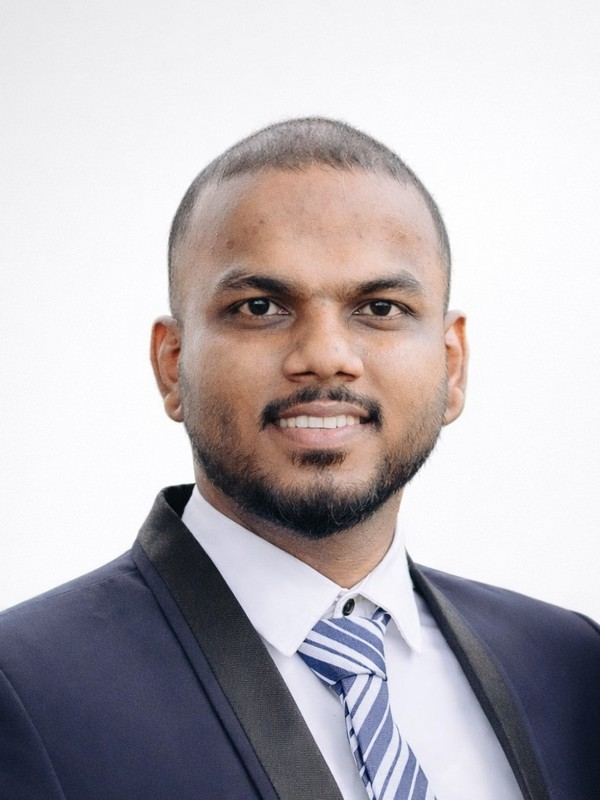
\includegraphics[width=2.75cm]{photo.jpg}
  \end{minipage}%
  \fi
  \par\vspace{3pt}
}
\newcommand{\cvsep}{\hspace{5pt}\textbullet\hspace{5pt}}

% Entry lists
\newcommand{\cvliststart}{\begin{itemize}[leftmargin=0.25cm, label={}, itemsep=3pt, topsep=0pt, parsep=0pt]}
\newcommand{\cvlistend}{\end{itemize}}

% \cventry{organisation}{location}{role or degree}{dates}
\newcommand{\cventry}[4]{%
  \item
  \begin{tabular*}{\linewidth}[t]{l@{\extracolsep{\fill}}r}
    \textbf{#1} & {\small #2} \\
    \textit{\small #3} & \textit{\small #4} \\
  \end{tabular*}\nopagebreak\vspace{-2pt}
}

% \cvproject{name}{technologies}{year}
\newcommand{\cvproject}[3]{%
  \item
  \begin{tabular*}{\linewidth}[t]{l@{\extracolsep{\fill}}r}
    {\small\textbf{#1} $|$ \textit{#2}} & \textit{\small #3} \\
  \end{tabular*}\nopagebreak\vspace{-2pt}
}

% \cvgroup{label}: sub-heading inside the project list
\newcommand{\cvgroup}[1]{\item[] \vspace{1pt}{\small\bfseries\itshape #1}\vspace{-1pt}}

% Bullet points under an entry
\newcommand{\cvpointsstart}{\begin{itemize}[leftmargin=0.45cm, label=\textbullet, itemsep=0.5pt, topsep=1pt, parsep=0pt]\small}
\newcommand{\cvpointsend}{\end{itemize}}

% \cvline{label}{text}: one line in the skills-style sections
\newcommand{\cvline}[2]{\item {\small \textbf{#1:} #2}}


\begin{document}

% ---------------------------------------------------------------- HEADER
\cvheader
  {Amberg, Germany \cvsep Nationality: Sri Lankan \cvsep Phone: \mbox{\cvphone}}
  {Email: \mbox{\href{mailto:\cvemail}{\cvemail}} \cvsep GitHub: \mbox{\href{https://\cvgithub}{\cvgithub}}}
  {LinkedIn: \mbox{\href{https://www.\cvlinkedin}{\cvlinkedin}}}
  {Portfolio: \mbox{\href{https://\cvportfolio/}{\cvportfolio}}}

% --------------------------------------------------------------- SUMMARY
\section{Professional Summary}
{\small
AI engineer and M.Sc.\ student in Artificial Intelligence for Industrial Applications with a B.Sc.\ in Mechanical
Engineering. AI and Automation Werkstudent at syskomp gehmeyr GmbH, with earlier industry experience in aviation
design and production automation. Focus on computer vision, LLMs/NLP and machine learning for industrial processes.
Strong in Python and PyTorch, with an emphasis on rigorous evaluation and models that can be deployed (ONNX export,
edge-ready rule models, small GPUs).
}

% ------------------------------------------------------------ EXPERIENCE
\section{Work Experience}
\cvliststart

  \cventry{syskomp gehmeyr GmbH}{Amberg, Germany}
          {AI and Automation Werkstudent (working student), part-time}{10/2026 -- present}
  \cvpointsstart
    \item Apply AI methods to engineering and industrial workflows in a mechanical engineering environment.
    \item Build and evaluate Python prototypes with an emphasis on traceable, validated results.
    \item Work with engineering colleagues to turn requirements into practical AI tooling.
  \cvpointsend

  \cventry{KNSI Aviation Engineering}{Negombo, Sri Lanka}
          {Design Engineer, full-time}{08/2023 -- 09/2024}
  \cvpointsstart
    \item Managed compliance data workflows and technical documentation with SQL and Excel to aviation standards.
    \item Built automated SQL/Excel reporting templates that cut weekly reporting time by 30\,\%.
    \item Analysed production data to optimise workflows, raising process efficiency by 40\,\%.
    \item Led the digitalisation of legacy documentation for faster cross-department data access.
  \cvpointsend

  \cventry{CBL Group (Ceylon Biscuits Limited)}{Pannipitiya, Sri Lanka}
          {Internship Trainee, Mechatronics \& Data}{02/2022 -- 11/2022}
  \cvpointsstart
    \item Contributed to process optimisation through data-driven solutions and automation projects.
    \item Supported end-of-line automation with articulated and parallel robots.
    \item Designed and prototyped 3D-printed automation components, reducing external sourcing costs and lead times.
    \item Deployed IoT sensors for real-time monitoring of production assets as groundwork for predictive maintenance.
  \cvpointsend

\cvlistend

% ------------------------------------------------------------- EDUCATION
\section{Education}
\cvliststart

  \cventry{OTH Amberg-Weiden (Technical University of Applied Sciences)}{Amberg, Germany}
          {M.Sc.\ Artificial Intelligence for Industrial Applications}{03/2025 -- present (expected 2027)}
  \cvpointsstart
    \item Modules: Computer Vision, Deep Vision, Deep Learning, NLP \& Information Retrieval, Autonomous Robotics,
          AI Security \& Privacy, Machine Learning, Industry 4.0.
  \cvpointsend

  \cventry{Preparation for Master's studies in Germany}{Sri Lanka / Germany}
          {Visa process, relocation and German language course}{10/2024 -- 02/2025}

  \cventry{University of Sri Jayewardenepura}{Sri Lanka}
          {B.Sc.\ (Hons) Mechanical Engineering, Minor in Mechatronics \textup{(GPA 3.27 / 4.0)}}{11/2019 -- 05/2023}
  \cvpointsstart
    \item Thesis: CNN surrogate model that predicts the aerodynamic drag of 2D shapes from images, replacing CFD runs.
    \item Project: design and build of a CoreXY 3D printer integrating mechanical design and machine learning.
  \cvpointsend

\cvlistend

% ---------------------------------------------------------------- SKILLS
\section{Technical Skills}
\cvliststart
  \cvline{Programming \& Tools}{Python (advanced), C++, SQL, Git/GitHub, REST APIs, pytest, Jupyter, LaTeX}
  \cvline{ML \& Deep Learning}{PyTorch, TensorFlow/Keras, scikit-learn, XGBoost, LightGBM, CatBoost, Optuna, CNN, RNN}
  \cvline{Computer Vision}{OpenCV, YOLOv8, object detection, semantic segmentation (U-Net, DeepLabV3+), Vision Transformers, Grad-CAM, ONNX}
  \cvline{NLP \& Generative AI}{Hugging Face Transformers, LLMs (Qwen, Llama, GPT), fine-tuning (LoRA/PEFT), RAG, LangChain, agentic workflows, SciBERT, LayoutLMv3, Tesseract OCR}
  \cvline{Robotics \& Industry 4.0}{Webots, SLAM, path planning (A*), PID control, MQTT, digital twins, IoT}
  \cvline{Data \& Backend}{pandas, NumPy, Matplotlib, Seaborn, MongoDB, Power BI, ETL pipelines, Weights \& Biases}
  \cvline{Mechanical Engineering}{CAD/CAM, SolidWorks, CFD simulation, 3D printing, mechatronics}
\cvlistend

% -------------------------------------------------------------- PROJECTS
\section{Projects}
\cvliststart

  \cvgroup{Industrial AI \& Computer Vision}

  \cvproject{X-ray Casting Defect Detection}{YOLOv8, OpenCV, ONNX}{2026}
  \cvpointsstart
    \item Fine-tuned YOLOv8n to detect pores, inclusions and shrinkage cavities in GDXray X-ray images of aluminium
          castings with a series-level split: test mAP50 0.545, precision 0.748.
    \item Failure analysis by defect size and a CLAHE ablation; ONNX export with identical detections at 60 ms per
          image on CPU.
  \cvpointsend

  \cvproject{Corrosion Segmentation: U-Net vs DeepLabV3+}{PyTorch, segmentation-models-pytorch}{2026}
  \cvpointsstart
    \item Pixel-level segmentation of four corrosion condition states on steel bridge inspection photos: mean IoU
          0.523; U-Net is clearly better on the safety-critical Severe class (IoU 0.325 vs 0.266).
  \cvpointsend

  \cvproject{CNN Surrogate Model for Aerodynamic Drag (B.Sc.\ thesis)}{TensorFlow, Keras, CFD}{2023}
  \cvpointsstart
    \item CNN that predicts the drag coefficient of 2D shapes from images in milliseconds instead of a CFD run;
          trained on 12,000 simulated shapes after comparing 7 architectures (validation MSE 0.0017).
    \item 0.06--2.77\,\% relative error on unseen real shapes, including NACA airfoils, against SolidWorks Flow
          Simulation.
  \cvpointsend

  \cvproject{Industrial Production Analytics Dashboard}{Power BI, DAX, Power Query, SQL}{2025}
  \cvpointsstart
    \item Power BI dashboards on star-schema models with automated ETL pipelines to track manufacturing KPIs.
  \cvpointsend

  \cvproject{Stacking Ensemble \& Edge-Ready Rule Model}{XGBoost, LightGBM, CatBoost, Optuna}{2025/26}
  \cvpointsstart
    \item Optuna-tuned stacking ensemble with R\textsuperscript{2} 0.848 on a 273-feature regression task; derived
          three if-else rules (R\textsuperscript{2} 0.915) that run on an edge device without ML libraries.
  \cvpointsend

  \cvproject{Pneumonia Detection: CNN vs ViT vs Hybrid}{PyTorch, timm, Grad-CAM}{2026}
  \cvpointsstart
    \item Compared ResNet-50, ViT-Base and TinyViT under identical conditions (5-fold CV ensembles): TinyViT reached
          94.9\,\% test accuracy (F1 0.948); assessed how faithful the Grad-CAM explanations are.
  \cvpointsend

  \cvproject{Digital IR Thermometer Simulation}{Python, NumPy, signal processing}{2025}
  \cvpointsstart
    \item Physics-based sensor simulation (noise, drift, emissivity bias, spikes) with filtering and outlier rejection.
  \cvpointsend

  \cvgroup{LLMs, NLP \& Document AI}

  \cvproject{Removing Jailbreak Backdoors from LLMs}{PyTorch, Hugging Face, LoRA/PEFT}{2026}
  \cvpointsstart
    \item Removed a known backdoor from Qwen2.5-1.5B with four-group hybrid supervised fine-tuning on a single 8 GB
          GPU: attack success rate reduced from 95\,\% to 1.7\,\% at 84\,\% benign accuracy (6.4\,\% out of distribution).
    \item Mechanistic analysis with linear probes shows the trigger is still detected (about 97\,\%): the defence
          changes the reaction, it does not erase the trigger.
  \cvpointsend

  \cvproject{QuantumCircuit Dataset Builder}{SciBERT, Transformers, BeautifulSoup, PyMuPDF}{2025/26}
  \cvpointsstart
    \item Automated pipeline that mines arXiv papers for quantum-circuit figures; fine-tuned SciBERT caption
          classifier (F1 0.954) producing 250 metadata records and 160 extracted images for image-to-text training.
  \cvpointsend

  \cvproject{LayoutLMv3 Form Understanding}{LayoutLMv3, Hugging Face, Tesseract OCR}{2026}
  \cvpointsstart
    \item Fine-tuned LayoutLMv3 for key-value extraction from scanned forms (FUNSD): entity-level F1 0.896.
  \cvpointsend

  \cvgroup{Robotics \& Industry 4.0}

  \cvproject{Autonomous ROSbot Maze Navigation}{Webots, SLAM, A*, PID, OpenCV}{2026}
  \cvpointsstart
    \item ROSbot that explores unknown mazes with LiDAR and depth-camera mapping, frontier exploration, A* planning
          and PID control; completed 4 of 5 mazes end to end, fastest full run 54 seconds.
  \cvpointsend

  \cvproject{ALIA-Delivery: Hospital Robot Digital Twin}{Webots, MQTT, Flask, A*}{2025}
  \cvpointsstart
    \item Digital twin of a hospital floor (team project): a TurtleBot3 receives delivery orders from a Flask control
          centre over MQTT, plans A* routes and drives to the patient's room.
  \cvpointsend

  \cvproject{CoreXY 3D Printer}{mechatronics, CAD/CAM, firmware}{B.Sc.\ project}
  \cvpointsstart
    \item Designed and built a CoreXY 3D printer from scratch: mechanical design, kinematics and firmware.
  \cvpointsend

  \cvgroup{Data Analysis}

  \cvproject{Study Program Intelligence}{Python, pandas, Monte Carlo, MCDA}{2026}
  \cvpointsstart
    \item Reproducible analysis of which new degree programme would attract the most students to OTH Amberg-Weiden:
          multi-criteria decision analysis under uncertainty with 10,000 Monte Carlo draws.
  \cvpointsend

  \cvproject{Students' Social Media Addiction: EDA}{pandas, Seaborn, Matplotlib}{2025}
  \cvpointsstart
    \item Exploratory analysis of 705 students from 110 countries; daily usage correlates with sleep at r = $-$0.79.
  \cvpointsend

\cvlistend

% ---------------------------------------------------------- CERTIFICATES
\section{Certifications \& Training}
\cvliststart
  \cvline{09/2025}{Bavarian-Czech AI Summer School, ``Niryo in Action: Controlling Robots with LLMs'' (32 hours), Speinshart, Germany}
  \cvline{DeepLearning.AI}{Deep Learning Specialization; Natural Language Processing Specialization (4 courses); AI for Medicine Specialization (3 courses)}
  \cvline{Talk}{``Adaptive-RAG'' (NAACL 2024 paper): 25-minute scientific talk, AI Conference module, OTH Amberg-Weiden, summer 2026}
\cvlistend

% ------------------------------------------------------------- LANGUAGES
\section{Languages}
\cvliststart
  \item {\small \textbf{English:} C1 (professional working level) \cvsep \textbf{German:} B1 (actively improving) \cvsep \textbf{Sinhala:} native language}
\cvlistend

% ------------------------------------------------------- EXTRACURRICULAR
\section{Leadership \& Activities}
\cvliststart
  \cvline{Entrepreneurship}{VYROBA TECHS: built a CoreXY 3D printer and ran a small custom-parts business during the pandemic}
  \cvline{Football}{player at FC Amberg; former captain of the faculty and university teams; University Colours Award for sports excellence (2022)}
\cvlistend

\end{document}
